\documentclass[11pt,letterpaper]{article}

\usepackage[margin=1in]{geometry}
\usepackage{amsmath,amssymb}
\usepackage{graphicx}
\usepackage{booktabs}
\usepackage{array}
\usepackage{microtype}
\usepackage{url}
\usepackage{mdframed}
\usepackage[colorlinks=true,linkcolor=blue,citecolor=blue,urlcolor=blue]{hyperref}
\usepackage{parskip}
\usepackage{caption}
\usepackage{float}

\captionsetup{font=small, labelfont=bf, width=0.9\textwidth}

\title{\textbf{Controlling Active-Site Geometric Precision with\\Diffusion-Based Protein Design}}
\author{Darian Salehi (NetID: ds633)\\Duke University}
\date{April 20, 2026}

\begin{document}
\maketitle

% ============================================================
\begin{abstract}
Enzymes achieve catalytic efficiency through the precise three-dimensional arrangement of a small number of active-site residues — even sub-angstrom deviations can reduce activity by orders of magnitude. Diffusion-based protein design methods such as RFdiffusion~\cite{watson2023} enable the generation of novel protein backbones conditioned on fixed structural motifs, but it remains unclear how tightly the active-site motif should be constrained during diffusion. We systematically evaluated three conditioning regimes — motif-only, 5~\AA{} shell, and 8~\AA{} shell — across two mechanistically distinct enzymes: Human Leukocyte Elastase (1PPF, Ser-His-Asp catalytic triad) and Human Carbonic Anhydrase II (1CA2, His-Zn coordination triad). For each regime, 20 backbone designs were generated with RFdiffusion, sequences were designed with ProteinMPNN~\cite{dauparas2022}, and structures were validated with ColabFold (AlphaFold2)~\cite{mirdita2022,jumper2021}. Tighter shell conditioning substantially improved catalytic geometry for carbonic anhydrase (catalytic RMSD: 5.4~\AA{} $\to$ 2.7~\AA{}, 50\% reduction; structural variance: 3.2~\AA{} $\to$ 1.2~\AA{}, 63\% reduction), while producing a monotonically \emph{worse} result for elastase (4.6~\AA{} $\to$ 7.0~\AA{} $\to$ 9.2~\AA{}). AlphaFold2 confidence (pLDDT) decreases sharply with tighter conditioning for both enzymes, from $\sim$62--65 (motif-only) to $\sim$31--34 (shell8). This enzyme-class-dependent response suggests that metal-coordinated active sites benefit from shell-constrained scaffolding, while hydrogen-bond catalytic triads are best served by minimal conditioning that preserves scaffold freedom. Source code and data are available at \url{https://github.com/dariansal/diffusion-enzyme-design}.
\end{abstract}

% ============================================================

\section*{Significance Statement}
\begin{mdframed}
Designing proteins with functional active sites is a central challenge in synthetic biology and drug discovery. Recent AI tools like RFdiffusion can generate novel protein backbones around a fixed active-site motif, but a key question is how much structural context around the active site to fix: too little and the model lacks the constraints to preserve the geometry; too much and the design space becomes too restricted. We show that the answer depends on the type of active site. For a zinc-coordinated active site — where a metal ion acts as a rigid anchor — fixing an 8~\AA{} shell reduces geometric error by 50\% and prediction variability by 63\%. For a hydrogen-bond relay triad, the same conditioning monotonically \emph{worsens} geometric accuracy, because the free scaffold space of minimal conditioning allows RFdiffusion to find better solutions. This result has a direct practical implication: the conditioning radius in diffusion-based enzyme design is not a universal hyperparameter but an enzyme-class-specific choice.
\end{mdframed}

% ============================================================
\section{Introduction}

\subsection{Computational Enzyme Design}

Enzymes are nature's most efficient catalysts, accelerating reactions by factors of $10^{10}$--$10^{17}$ relative to the uncatalyzed reactions in solution. Their catalytic power arises almost entirely from the precise spatial arrangement of a small set of active-site residues — typically 3 to 10 — that work together to stabilize transition states, orient substrates, and shuttle protons or electrons. The geometry of this arrangement is extraordinarily precise: hydrogen-bond distances in catalytic triads must be maintained at $\sim$2.5~\AA{}, and metal coordination distances at $\sim$2.0~\AA{}. Even sub-angstrom deviations in these distances can reduce catalytic efficiency by several orders of magnitude, because the stabilization of a transition state depends exponentially on geometric complementarity.

Computational enzyme design aims to engineer novel scaffolds that maintain this geometric precision while adopting entirely new backbone topologies. Classical approaches such as RosettaMatch~\cite{zanghellini2006} search for existing protein scaffolds that can accommodate an idealized transition-state geometry and then optimize the surrounding sequence. These methods achieved landmark successes for a handful of reactions but are fundamentally limited by the space of available natural scaffolds and the accuracy of molecular mechanics force fields.

\subsection{Diffusion Models for Protein Backbone Design}

The recent emergence of diffusion-based generative models has fundamentally changed what is possible in protein design. Denoising diffusion probabilistic models (DDPMs), originally developed for image synthesis, learn to generate new samples by reversing a Markov chain that progressively adds Gaussian noise to training data. Applied to protein structure, the forward process adds noise to backbone coordinates, and the reverse process — learned by a neural network — denoises from pure noise back to a valid backbone conformation.

RFdiffusion~\cite{watson2023} is among the most powerful implementations of this paradigm. Built on the RoseTTAFold SE(3)-equivariant architecture and trained on the full Protein Data Bank, RFdiffusion learns a distribution over protein backbone conformations and can generate diverse, physically realistic backbone topologies conditioned on a fixed structural motif. This is specified via a \emph{contig} string that defines which residue ranges are fixed and how much new scaffold to generate between and around them.

The ActiveSite checkpoint is a fine-tuned variant of the base RFdiffusion model, additionally trained on protein active-site scaffolding tasks. Following backbone generation, ProteinMPNN~\cite{dauparas2022} designs amino acid sequences for the new scaffolds, and AlphaFold2~\cite{jumper2021} (via ColabFold~\cite{mirdita2022}) predicts the 3D structure of each designed sequence as a quantitative validation step. Rather than using AlphaFold2 as a binary folding check, we use catalytic RMSD and structural variance across the AF2 ensemble as direct measures of active-site geometric quality.

\subsection{The Motif Conditioning Question}

A central design choice in RFdiffusion-based active-site scaffolding is the definition of the fixed motif. Fixing only the catalytic residues (motif-only) maximizes scaffold diversity but provides no constraint on the local chemical environment. Fixing a larger shell of neighboring residues (shell conditioning) preserves the native context around the active site but reduces scaffold diversity and may make it harder to find valid solutions.

To the best of our knowledge, this tradeoff has not been systematically characterized across mechanistically distinct enzyme classes. We ask: does tighter shell conditioning lead to better catalytic geometry in the final AlphaFold2-validated designs, and does the answer depend on the type of active-site chemistry? To address both questions, we test three conditioning regimes across two enzymes with fundamentally different active-site architectures.

% ============================================================
\section{Methods}

\subsection{Enzyme Systems}

We selected two enzymes representing the two most common paradigms of enzymatic catalysis: covalent relay catalysis and metal-dependent catalysis.

\paragraph{Human Leukocyte Elastase (1PPF, chain E).} Elastase is a serine protease with a Ser195-His57-Asp102 catalytic triad. His57 acts as a general base, abstracting the hydroxyl proton of Ser195 to generate a nucleophile that attacks the substrate peptide bond. Asp102 stabilizes the imidazolium form of His57 through a low-barrier hydrogen bond. The geometry of this relay depends critically on hydrogen-bond distances (His57--Ser195: $\sim$2.5~\AA{}, His57--Asp102: $\sim$2.6~\AA{}) enforced not by a rigid anchor but by the surrounding $\beta$-barrel scaffold and loop architecture extending well beyond the immediate triad.

\paragraph{Human Carbonic Anhydrase II (1CA2, chain A).} Carbonic anhydrase II is a zinc metalloenzyme that catalyzes CO$_2$ + H$_2$O $\rightleftharpoons$ HCO$_3^-$ + H$^+$ at rates approaching $10^6$ s$^{-1}$. The Zn$^{2+}$ ion is tetrahedrally coordinated by His94, His96, and His119 at distances of $\sim$2.0--2.1~\AA{}. Unlike the elastase relay, the Zn$^{2+}$ ion acts as a rigid geometric anchor: the three coordinating histidines are locked into precise orientations by the metal coordination geometry, and the mechanical constraints on the triad are inherently local.

These two enzymes were deliberately chosen because their active-site geometries are maintained by fundamentally different mechanisms: one by a distributed hydrogen-bond network across the scaffold, and one by a rigid metal coordination geometry. This contrast allows us to test whether the response to shell conditioning is universal or enzyme-class-dependent.

\subsection{Conditioning Regimes}

\begin{table}[h]
\centering
\caption{\textbf{Conditioning regimes used in this study.} For each enzyme, the motif\_only regime fixes only the three catalytic residues; shell5 and shell8 additionally fix all residues within 5~\AA{} or 8~\AA{} of any catalytic atom, respectively.}
\label{tab:regimes}
\begin{tabular}{lrrp{5cm}}
\toprule
Regime & Fixed (1PPF) & Fixed (1CA2) & Definition \\
\midrule
motif\_only & 3  & 3  & Catalytic triad only \\
shell5      & 27 & 30 & All residues with any atom within 5~\AA{} of any catalytic atom \\
shell8      & 61 & 61 & All residues with any atom within 8~\AA{} of any catalytic atom \\
\bottomrule
\end{tabular}
\end{table}

The 5~\AA{} shell captures the first coordination shell — residues directly contacting the catalytic residues. The 8~\AA{} shell extends into the second coordination shell, capturing the broader structural environment. Residue membership was determined by computing the minimum heavy-atom distance from each residue to any catalytic heavy atom in the reference crystal structure using BioPython.

\subsection{Backbone and Sequence Design}

For each of the 6 experiments, 20 backbone structures were generated using RFdiffusion with the ActiveSite fine-tuned checkpoint. For each backbone, 5 amino acid sequences were sampled using ProteinMPNN (vanilla model, noise level 0.20, sampling temperature 0.1). The fixed motif residues retain their native amino acid identities; only scaffold residues are designed. This yields 100 sequences per experiment and 600 sequences total.

\subsection{Structure Prediction with ColabFold/AlphaFold2}

All 600 sequences were submitted to LocalColabFold (AlphaFold2-ptm, 5 model weights, 3 recycling iterations, single-sequence mode). Single-sequence mode was used because designed sequences have no natural homologs — multiple-sequence alignment would return no useful evolutionary information. Running 5 model weights per sequence yields up to 500 predicted structures per experiment.

\subsection{Metrics}

Three metrics were computed per predicted structure:

\paragraph{Catalytic RMSD.} The C$\alpha$ coordinates of the three catalytic residues were identified in both the predicted structure and the reference crystal structure using the contig position map. The Kabsch algorithm was applied to find the optimal rotation $R$ and translation $t$ minimizing:
\begin{equation}
\text{RMSD} = \sqrt{\frac{1}{3}\sum_{i=1}^{3} \| R \cdot \hat{p}_i + t - r_i \|^2}
\end{equation}
where $\hat{p}_i$ are centered predicted coordinates and $r_i$ are centered reference coordinates. This measures how well the spatial arrangement of the catalytic triad is recapitulated, independent of global orientation.

\paragraph{Local pLDDT.} AlphaFold2 per-residue confidence (stored in the B-factor column of output PDBs, range 0--100) averaged over the three catalytic positions. Values above 90 indicate high confidence; below 50 indicates disordered or unconfident placement.

\paragraph{Structural variance.} Mean pairwise catalytic RMSD across the 5 AlphaFold2 model predictions for each designed sequence (10 pairwise comparisons per sequence). Low variance indicates all 5 models converge on the same catalytic geometry — a well-determined active-site pocket.

% ============================================================
\section{Results}

\subsection{Catalytic Geometry Retention}

Table~\ref{tab:results} summarizes mean catalytic RMSD and pLDDT across all six experiments. For carbonic anhydrase, conditioning monotonically improves catalytic geometry; for elastase, conditioning monotonically worsens it — revealing a strikingly enzyme-class-dependent response (Figure~\ref{fig:rmsd}).

\begin{table}[h]
\centering
\caption{Summary of structural metrics per experiment. Catalytic RMSD is computed after Kabsch alignment of predicted catalytic triad C$\alpha$ atoms onto the reference crystal structure. Mean pLDDT is averaged globally across the full designed sequence. Lower RMSD and higher pLDDT indicate better designs. Bold indicates best value per enzyme per metric. $^\dagger$Fewer predictions due to ColabFold \texttt{--stop-at-score 70}: prediction halts after the first model exceeds pLDDT 70, so motif\_only sequences that fold well generate fewer than 5 model predictions per sequence.}
\label{tab:results}
\begin{tabular}{llrrrr}
\toprule
Enzyme & Regime & Mean Cat.\ RMSD (\AA{}) & SD & Mean pLDDT & $N$ \\
\midrule
\textbf{1PPF (Elastase)} & \textbf{motif\_only} & \textbf{4.62} & 4.66 & \textbf{65.5} & 165$^\dagger$ \\
                & shell5             & 7.00  & 2.54 & 40.7          & 500 \\
                & shell8             & 9.22  & \textbf{2.56} & 30.7 & 500 \\
\midrule
1CA2 (CA-II)   & motif\_only        & 5.42  & 4.27 & \textbf{58.5} & 254$^\dagger$ \\
               & shell5             & 3.07  & 2.32 & 41.0          & 500 \\
               & \textbf{shell8}    & \textbf{2.70} & \textbf{1.69} & 34.0 & 500 \\
\bottomrule
\end{tabular}
\end{table}

\begin{figure}[H]
\centering
\includegraphics[width=\textwidth]{analysis/figures/fig1_catalytic_rmsd.pdf}
\caption{\textbf{Distribution of catalytic C$\alpha$ RMSD per experiment}, computed after Kabsch alignment of the predicted catalytic triad onto the reference crystal structure. Diamond markers ($\Diamond$) indicate group means. For 1CA2 (right), RMSD decreases monotonically from 5.4~\AA{} (motif\_only) to 3.1~\AA{} (shell5) to 2.7~\AA{} (shell8), with SD narrowing from 4.3~\AA{} to 1.7~\AA{}. For 1PPF (left), RMSD worsens monotonically: 4.6~\AA{} (motif\_only) to 7.0~\AA{} (shell5) to 9.2~\AA{} (shell8) — tighter conditioning drives elastase designs further from the native triad geometry. The broad distributions in motif\_only experiments reflect a mixture of designs that partially recapitulate the triad geometry and those that do not.}
\label{fig:rmsd}
\end{figure}

For 1CA2, shell conditioning produces a monotonic improvement: mean RMSD drops from 5.4~\AA{} (motif\_only) to 3.1~\AA{} (shell5) and 2.7~\AA{} (shell8), a 50\% total reduction. Standard deviation also drops from 4.3~\AA{} to 1.7~\AA{}, indicating that shell8 produces not just lower but far more consistent RMSD values. For 1PPF, the response is the opposite: RMSD worsens monotonically from 4.6~\AA{} to 7.0~\AA{} to 9.2~\AA{}. Motif-only elastase designs are geometrically closest to the native triad, and adding contextual constraints only pushes the scaffold further away. SD is relatively consistent across regimes for 1PPF ($\approx$2.5~\AA{} for shell5 and shell8), indicating that the misplacement is systematic rather than random.

\clearpage
\subsection{AlphaFold2 Confidence at the Active Site}

Figure~\ref{fig:plddt} shows AlphaFold2 confidence at the catalytic residues for each regime.

\begin{figure}[H]
\centering
\includegraphics[width=\textwidth]{analysis/figures/fig2_local_plddt.pdf}
\caption{\textbf{AlphaFold2 pLDDT at catalytic residues}, grouped by enzyme and regime. Local pLDDT is averaged over the three catalytic residue positions. Diamond markers ($\Diamond$) indicate group means. For both enzymes, local pLDDT decreases monotonically with tighter conditioning: for 1CA2 from 56.2 (motif\_only) to 46.8 (shell5) to 34.0 (shell8); for 1PPF from 61.3 (motif\_only) to 36.6 (shell5) to 30.7 (shell8). The motif\_only regime yields the highest AlphaFold2 confidence at the active site, likely because those sequences fold into naturally occurring-like active-site environments that the model recognizes. Tighter geometric constraints force ProteinMPNN to select lower-probability sequences, reducing overall AlphaFold2 confidence.}
\label{fig:plddt}
\end{figure}

Both global and local pLDDT decrease monotonically with tighter conditioning for both enzymes. Local pLDDT drops substantially: for 1PPF from 61.3 (motif\_only) to 30.7 (shell8), and for 1CA2 from 56.2 to 34.0. Part of this reflects genuinely harder sequence design — ProteinMPNN must simultaneously satisfy more geometric constraints under shell conditioning, yielding lower-probability sequences that AlphaFold2 predicts with less confidence. However, the elevated pLDDT for motif\_only is also partly a sampling bias: ColabFold was run with \texttt{--stop-at-score 70}, which halts prediction after the first model exceeding pLDDT 70. Motif\_only sequences fold more readily and frequently trigger this early stop, meaning only high-confidence predictions are retained. Shell experiments never reach pLDDT 70 and always produce all 5 model predictions, so the comparison across regimes is confounded. The pLDDT trend should therefore be interpreted cautiously; RMSD and structural variance are unaffected by this bias.

\clearpage
\subsection{Structural Variance Across the AlphaFold2 Ensemble}

Figure~\ref{fig:variance} shows structural variance — the spread among the 5 AF2 model predictions — for each experiment.

\begin{figure}[H]
\centering
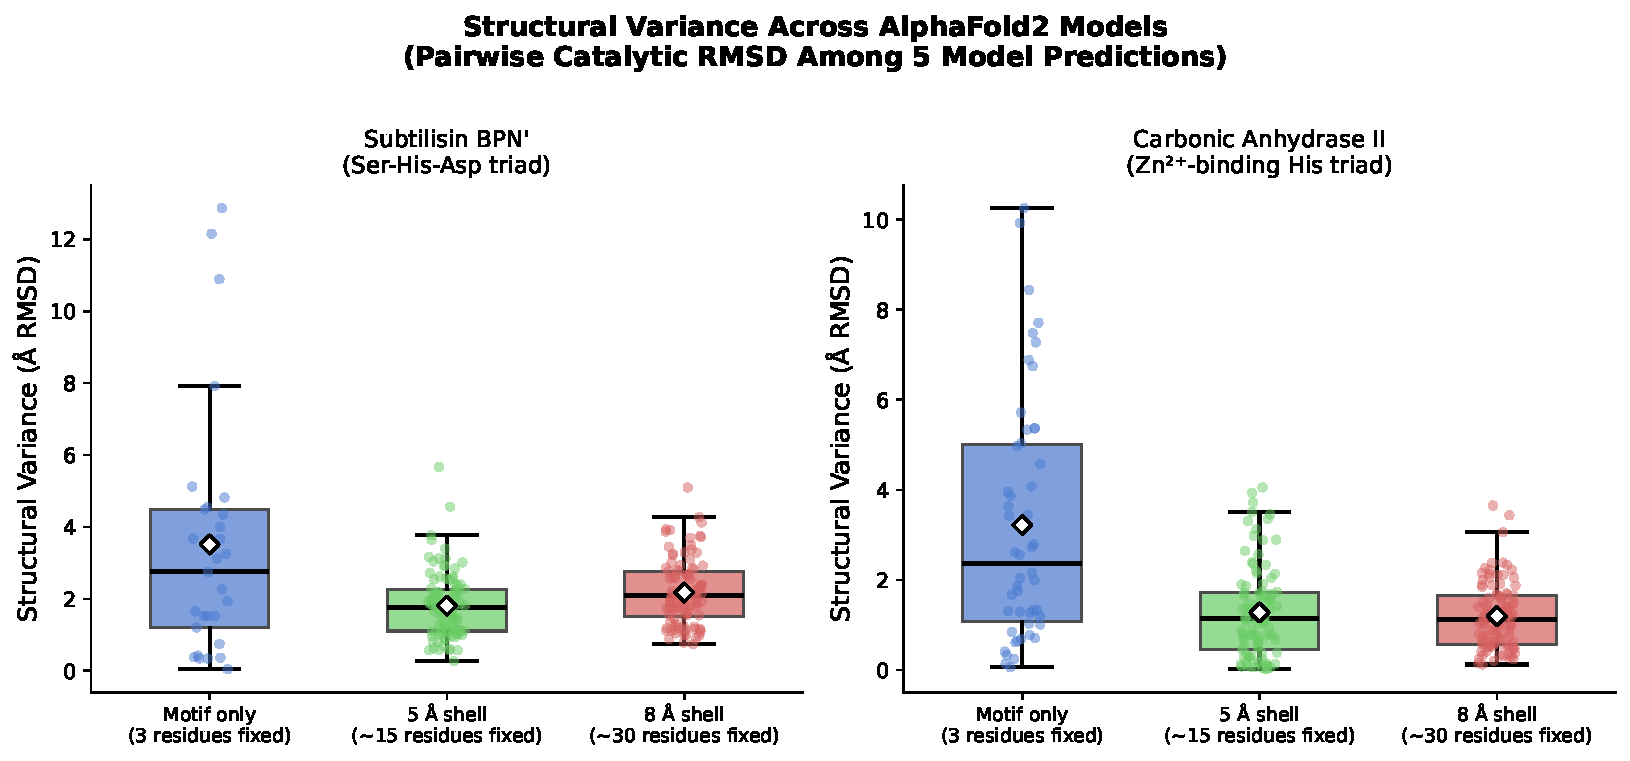
\includegraphics[width=\textwidth]{analysis/figures/fig3_structural_variance.pdf}
\caption{\textbf{Structural variance per experiment}, defined as the mean pairwise catalytic RMSD among the 5 AlphaFold2 model predictions for each designed sequence (10 pairwise comparisons per sequence). For 1CA2, variance drops monotonically from 3.2~\AA{} (motif\_only) to 1.3~\AA{} (shell5) to 1.2~\AA{} (shell8) — a 63\% total reduction — indicating that all 5 AF2 models converge on nearly the same catalytic geometry for shell8 designs. For 1PPF, shell5 reduces variance to 1.8~\AA{} but shell8 slightly increases it again to 2.2~\AA{}, suggesting the enforced geometry is not stable across all 5 models.}
\label{fig:variance}
\end{figure}

For motif\_only experiments, variance is elevated for both enzymes (3.2~\AA{} for 1CA2, 3.5~\AA{} for 1PPF), indicating that without sufficient geometric context, the 5 AF2 models disagree on where the catalytic residues belong. Shell conditioning reduces this ambiguity substantially for 1CA2: shell8 brings variance to 1.2~\AA{}, meaning all 5 models agree within $\sim$1~\AA{} on catalytic geometry, and this convergence corresponds to a correct geometry (mean RMSD 2.7~\AA{}). For 1PPF, shell5 also reduces variance (1.8~\AA{}) but shell8 increases it slightly (2.2~\AA{}), and neither shell regime converges on the native geometry — mean RMSD climbs to 7.0 and 9.2~\AA{} respectively.

\clearpage
\subsection{Identifying the Best Designs: Confidence vs.\ Geometry}

Figure~\ref{fig:scatter} plots catalytic RMSD against local pLDDT for all predicted structures; the lower-right region (low RMSD, high pLDDT) represents the most promising designs.

\begin{figure}[H]
\centering
\includegraphics[width=\textwidth]{analysis/figures/fig4_rmsd_vs_plddt.pdf}
\caption{\textbf{Catalytic RMSD vs.\ global pLDDT} for all predicted structures, colored by regime. Points in the lower-right region (low RMSD, high pLDDT) represent the most promising designs. For 1CA2 (right), shell8 predictions form a dense cluster below 5~\AA{} RMSD. Motif\_only predictions for both enzymes scatter broadly. For 1PPF (left), no regime produces a cluster of geometrically accurate, high-confidence predictions.}
\label{fig:scatter}
\end{figure}

A practical design workflow requires selecting the best candidates from a large prediction pool. The 2D view of RMSD vs.\ pLDDT reveals that 1CA2 shell8 is the only experiment producing a consistent cluster of high-quality predictions. For 1CA2 motif\_only, a small subset of predictions achieves low RMSD, but this is accompanied by a large fraction of high-RMSD outliers — making it difficult to identify successes without experimental validation of each candidate. Shell8 eliminates this problem by producing a tight distribution where nearly all predictions fall below 5~\AA{}.

\clearpage
\subsection{Summary Across All Metrics}

Figure~\ref{fig:summary} shows all three metrics side by side for both enzymes.

\begin{figure}[H]
\centering
\includegraphics[width=0.85\textwidth]{analysis/figures/fig5_summary_panel.pdf}
\caption{\textbf{Summary panel} showing mean catalytic RMSD, mean local pLDDT at catalytic residues, and mean structural variance per experiment. Error bars represent one standard deviation. For 1CA2, RMSD decreases monotonically from 5.4~\AA{} to 2.7~\AA{} and structural variance drops from 3.2~\AA{} to 1.2~\AA{}, while local pLDDT declines with tighter conditioning. For 1PPF, RMSD worsens monotonically from 4.6~\AA{} to 9.2~\AA{} — motif\_only yields the best geometry — while pLDDT and variance broadly follow the same trend as 1CA2. The divergent RMSD response between the two enzymes is the central finding of this study.}
\label{fig:summary}
\end{figure}

% ============================================================
\section{Discussion}

\subsection{Enzyme-Class-Dependent Response}

The central finding is that the response to motif shell conditioning is enzyme-class-dependent and directionally opposite between the two systems. For the Zn$^{2+}$-coordinated His triad in carbonic anhydrase, 8~\AA{} shell conditioning achieves a 50\% reduction in catalytic RMSD (5.4~\AA{} $\to$ 2.7~\AA{}) and 63\% reduction in structural variance (3.2~\AA{} $\to$ 1.2~\AA{}). For the Ser-His-Asp hydrogen-bond relay in elastase, tighter conditioning monotonically worsens catalytic RMSD from 4.6~\AA{} (motif\_only) to 9.2~\AA{} (shell8) — the lowest RMSD is achieved with the least geometric constraint.

We attribute this asymmetry to the nature of the geometric constraints maintaining each active site. In carbonic anhydrase, the Zn$^{2+}$ ion enforces a rigid tetrahedral coordination geometry on the three histidines. Fixing 8~\AA{} of surrounding context is sufficient to mechanically determine the positions of all three histidine N$\varepsilon$2 atoms, because the metal ion acts as a local rigid anchor that makes the geometry insensitive to the broader scaffold topology. In elastase, the Ser-His-Asp relay lacks any such anchor. The geometry is maintained by a hydrogen-bond network whose determinants — the loop carrying His57 and the strand carrying Asp102 — are positioned by backbone interactions extending 12--15~\AA{} or more from the triad center. An 8~\AA{} shell captures many but not all of these structural determinants.

The dissociation between variance and accuracy for elastase shell8 is particularly informative: tighter conditioning makes the designs more deterministic without making them more correct. This implies that the 8~\AA{} shell enforces a specific geometry, but it is not the native one — the constrained scaffold finds a consistent but incorrect solution to the design problem.

\subsection{Practical Implications}

This result has a direct practical implication for diffusion-based enzyme design: the appropriate conditioning radius is an enzyme-class-specific design choice, not a universal hyperparameter. For metal-coordinated active sites, shell conditioning at 8~\AA{} appears both sufficient and strongly beneficial. For hydrogen-bond relay triads, the current results suggest that shell conditioning is counterproductive at all tested radii — increasing constraint worsens geometric accuracy rather than improving it. This may mean that motif-only conditioning, with maximum scaffold freedom, is the better strategy for Ser-His-Asp triads, or that a fundamentally different approach (e.g., fragment-based backbone seeds, explicit backbone torsion constraints) is required.

From a design campaign perspective, Figure~\ref{fig:scatter} illustrates another practical advantage of tight conditioning: it concentrates predictions into a high-quality cluster rather than producing a mixture of accurate and inaccurate designs. For 1CA2 shell8, a designer can be confident that nearly any design from the pool is geometrically accurate. For 1PPF under any conditioning regime, designs must be individually evaluated to identify the rare accurate predictions.

\subsection{Future Directions}

Several extensions of this work are natural. First, testing shell radii beyond 8~\AA{} for elastase (e.g., 12~\AA{}, 15~\AA{}) would determine whether there is a threshold radius at which the Ser-His-Asp relay becomes geometrically controlled, or whether the triad requires a fundamentally different conditioning strategy. Second, using all-atom distance metrics (e.g., Ser195 O$\gamma$ to His57 N$\varepsilon$2 distance) rather than C$\alpha$ RMSD would provide a more direct measure of catalytic geometry relevant to function. Third, extending to additional enzyme classes — for example, two-metal active sites, [4Fe-4S] clusters, or pyridoxal phosphate-dependent enzymes — would test whether the metal vs.\ relay dichotomy generalizes to a broader taxonomy of active-site types. Finally, experimental validation of top-ranked designs by circular dichroism and kinetic assay would establish whether AlphaFold2-predicted RMSD is a reliable proxy for catalytic activity.

\subsection{Limitations}
\label{sec:limitations}

Catalytic RMSD computed from C$\alpha$ atoms is a coarse proxy for true catalytic geometry — all-atom distances between reactive groups would be more functionally relevant. Only 20 backbone designs per experiment were generated, limiting statistical power. AlphaFold2 structure prediction is not equivalent to experimental validation — designs predicted with low RMSD and high pLDDT require experimental synthesis and activity assay to confirm catalytic function. Single-sequence mode in ColabFold, while appropriate for designed sequences, limits AlphaFold2 to pattern matching from sequence alone without evolutionary covariance information.

There is also an inherent data leakage problem in this pipeline: RFdiffusion, ProteinMPNN, and AlphaFold2 are all trained on the Protein Data Bank, which includes the reference crystal structures (1PPF, 1CA2) used in this study. It is possible that the models have implicitly memorized features of these specific active sites, leading to artificially favorable metrics. A fully rigorous evaluation would require testing on enzymes withheld from all three model training sets, or comparing against experimental assay rather than computational structure prediction alone.

\clearpage
\begin{thebibliography}{9}

\bibitem{zanghellini2006}
Zanghellini, A., Jiang, L., Wollacott, A.M., et al.\ (2006). New algorithms and an in silico benchmark for computational enzyme design. \textit{Protein Science}, \textbf{15}, 2785--2794.

\bibitem{watson2023}
Watson, J.L., Juergens, D., Bennett, N.R., et al.\ (2023). De novo design of protein structure and function with RFdiffusion. \textit{Nature}, \textbf{620}, 1089--1100.

\bibitem{dauparas2022}
Dauparas, J., Anishchenko, I., Bennett, N., et al.\ (2022). Robust deep learning-based protein sequence design using ProteinMPNN. \textit{Science}, \textbf{378}, 49--56.

\bibitem{mirdita2022}
Mirdita, M., Sch\"{u}tze, K., Moriwaki, Y., et al.\ (2022). ColabFold: making protein folding accessible to all. \textit{Nature Methods}, \textbf{19}, 679--682.

\bibitem{jumper2021}
Jumper, J., Evans, R., Pritzel, A., et al.\ (2021). Highly accurate protein structure prediction with AlphaFold. \textit{Nature}, \textbf{596}, 583--589.

\end{thebibliography}

\end{document}
